%The transcription for prokaryote is composed of 4 steps:
%\begin{enumerate}
%  \item promoter search;
%  \item initiation;
%  \item elongation;
%  \item termination.
%\end{enumerate}




\subsubsection{Promoter search} Before binding to DNA, the RNA polymerase has to find it: it is called promoter search. It was generally admitted that a 3D-diffusion search was not enough as some search rate measure were above the 3D-diffusion possible rate. Some other mechanisms were proposed: 1D sliding along the DNA, 1D hoping and DNA intersegment jump. In \citep{Hal:09}, it is suggested however that the promoter search rate is consistent with a 3D diffusion rate.



\subsubsection{Initiation}
%\paragraph{Biological process}
The purpose of initiation is to locate precisely the Pribnow's box (TATAAT for $\sigma^{70}$ sigma factor) so that the RNA polymerase can bind to it. This binding is favoured by a sigma factor. A non-bounded RNA polymerase is composed of 4 sub-units ($2\alpha$, $\beta$, $\beta'$ and $\omega$): it is a core-enzyme. The initiation ends with the promoter clearance and eventually the release of the sigma factor. It follows the steps \citep{SdH:11}:
\begin{enumerate}
  \item a sigma factor binds to the core-enzyme becoming a holo-enzyme:
    $$
      \reactionRev{pRNA + \sigma^i}{pRNA\Sigma^i}{}{}
    $$
    There are several types of sigma factor and each of them increases the affinity of the holo-enzyme RNA polymerase to the specific promoter.
  \item The holo-enzyme then binds to a DNA promoter and forms a closed complex. This triggers a series of conformational changes collectively called 'izomerization':
      \begin{itemize}
        \item opens $~13$ bp from the -10 elements beyond the transcription start site for the sigma factor and -35 for the $\alpha$ sub-unit while the complex protects a 'footprint' of around 30 bp from nuclease digestion \citep{vHi:98};
        \item creates the initiation 'bubble' and a stable open complex after an unstable one.
      \end{itemize}
      It is summarized with the reactions:
    $$
      \left\{
        \begin{array}{l}
          \reactionIrr{pRNA\sigma^i + DNA}{cDpRNA\sigma^i}{}{} \\
          \reactionIrr{cDpRNA\sigma^i}{oDpRNA\sigma^i}{}{} \\
        \end{array}
      \right.
    $$
  \item The open complex then synthesizes nascent RNA and tries to leave the promoter site (promoter clearance). However, around 10 abortive initiations happens \citep{GoN:09} in mean before promoter clearance is really performed:
      $$
        \left\{
          \begin{array}{l}
            \reactionIrr{oDpRNA\sigma^i + \sum m_irNTP^i}{oDpRNA\sigma^i + nRNA}{}{} \\
            \reactionIrr{oDpRNA\sigma^i + \sum m_irNTP^i}{DpRNA\sigma}{}{} \\
          \end{array}
        \right.
        .
      $$
      The first reaction models the abortive initiation as the synthesis of the nascent RNA being apart from the DNA - RNA polymerase complex. Physicality, the nascent RNA is still inside the complex and goes away from the complex when the sigma factor is released. The second reaction models the promoter clearance with the nascent RNA still attached to the complex.
  \item The sigma factor is released. Physically, the sigma factor can be either released during the promoter clearance or during the beginning of elongation.
      $$
        \reactionIrr{DpRNA\sigma}{DpRNA}{}{} \\
      $$
      The trigger is not clear however it is released typically when the nascent RNA reaches a length of 12-15 nt.
\end{enumerate}

%\paragraph{Biological error} The authors are not aware of any biological error that can happen during initiation of transcription.







\subsubsection{Elongation}
%\paragraph{Biological process}
The elongation consists in binding the ribose NTP to each other and step forward:
\begin{enumerate}
  \item recruitment of the ribose NTP corresponding:
    $$
      \reactionRev{DpRNA + rNTP^i}{DpRNA^i}{}{} . \\
    $$
    A 'wrong' ribose NTP could be recruited at this step, or even a deoxyribose NTP [reference needed];
  \item binding of the recruited ribose NTP to the former one, catalyzed by a pair of \ce{Mg2+}:
    $$
      \reactionIrr{DpRNA^i + \ce{H2O}}{DpRNA^+ + PP_i}{\ce{Mg^2+}}{} ; \\
    $$
  \item translocation where the RNA polymerase step one base forward:
    $$
      \reactionIrr{DpRNA^+}{DpRNA}{}{} . \\
    $$
\end{enumerate}
The movement of the polymerase forms a Brownian ratchet motion. The elongation rate is around 6.2-20 bp/s. In competition to the step forward motion, there are:
\begin{itemize}
  \item pausing consists in the RNA polymerase to pause during some time but the mechanics are unclear. Promoter proximal pause also happens. \citep{LaW+:14} proposes a consensus sequence of 11 nt length for pausing detection. An early release of the nascent RNA transcript may happen during pausing;
  \item backtracking consists in the cleavage of 2 or more nucleotides. It seems to be a kind of proofreading. It is not clear when and how it happens;
  \item stalling consists in the RNA polymerase to wait, especially for rare ribose NTP to be recruited. Stalling is thought to help the folding of the nascent polypeptide chain [reference needed].
\end{itemize}


%\paragraph{Biological error} An early release of the nascent RNA transcript may happen, especially during pausing. Not the good rNTP



\subsubsection{Termination}
%\paragraph{Biological process}
For prokaryotes, there are two types of termination:
\begin{enumerate}
  \item Rho-independent or independent termination \citep{GuN:99,WaG:10}: nascent RNA forms a rich G-C hairpin followed by 7-9 U bases. This weakens the DNA - RNA polymerase complex. The force due to the hairpin is not enough though and some other mechanisms, which is performed by the binding of NusA, is needed \citep{HeB:08};
  \item Rho-dependent termination: a rho co-factor helps the termination. Two major models exist: $(i)$ the rho factor binds to the rut (rho utilization site of about 70 - 100 nucleotides) or rho binding site and then moves forward towards transcription stop point (tsp) region creating an hairpin; $(ii)$ the rho factor binds to the polymerase \citep{EDWN:10} and an hairpin is created while the polymerase elongates. In the tsp region, there are (potentially) several pause positions for the RNA polymerase in the absence of rho co-factor, the termination occurs at these stop positions.
\end{enumerate}


%\paragraph{Biological error} The authors are not aware of any biological error that can happen during termination of transcription.



\subsubsection{Others}

\paragraph{Transcript slippage} The phenomenon is illustrated in Figure \ref{fig:slippage} in the case where the RNA polymerase idles; forward and backward slippage are also described in \cite{ATM:10}.
\begin{figure}[!ht]
	\centering
	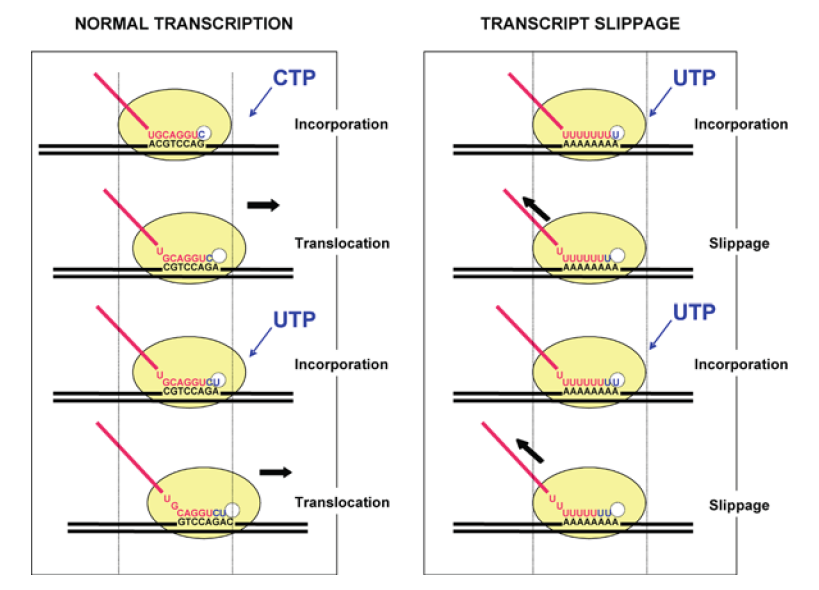
\includegraphics[width=0.8\linewidth]{figure/transcriptSlippage}
	\caption{Illustration of transcript slippage, from \cite{ATM:10}}
	\label{fig:slippage}
\end{figure}
It mainly occurs on homopolymeric tracts. Slippage can occur during initiation, elongation and termination, as well as during replication and translation. Slippage during transcription initiation plays a role in transcription regulation by abortive transcripts \cite{Tur:11}. Bacteria can take advantage of slippage in few ways as described in \cite{ATM:10}:
\begin{itemize}
  \item use a single mRNA to encode two proteins;
  \item restore a reading frame that would be otherwise be interrupted by the addition or deletion of a nucleotide.
\end{itemize}
